% !TEX TS-program = pdflatex
% !TEX encoding = UTF-8 Unicode

\documentclass[a4paper, titlepage=false, parskip=full-, 10pt]{scrartcl}

\usepackage[utf8]{inputenc}
\usepackage[T1]{fontenc}
\usepackage[english, ngerman]{babel}
\usepackage{babelbib}
\usepackage{hyperref}
\usepackage{listings}
\usepackage{framed}
\usepackage{color}
\usepackage{graphicx}
\usepackage[normalem]{ulem}
\usepackage{cancel}
\usepackage{amsmath}
\usepackage{amssymb}
\usepackage{amsthm}
\usepackage{algorithm}
\usepackage{algorithmic}
\usepackage{geometry}
\usepackage{subfigure}
\geometry{a4paper, top=20mm, left=35mm, right=25mm, bottom=40mm}

\newcounter{tasknbr}
\setcounter{tasknbr}{1}
\newenvironment{task}[1]{{\bf Aufgabe \arabic {tasknbr}\stepcounter{tasknbr}} (#1):\begin{enumerate}}{\end{enumerate}}
\newcommand{\subtask}[1]{\item[#1)]}

% Listings -----------------------------------------------------------------------------
\definecolor{red}{rgb}{.8,.1,.2}
\definecolor{blue}{rgb}{.2,.3,.7}
\definecolor{lightyellow}{rgb}{1.,1.,.97}
\definecolor{gray}{rgb}{.7,.7,.7}
\definecolor{darkgreen}{rgb}{0,.5,.1}
\definecolor{darkyellow}{rgb}{1.,.7,.3}
\lstloadlanguages{C++,[Objective]C,Java}
\lstset{
escapeinside={§§}{§§},
basicstyle=\ttfamily\footnotesize\mdseries,
columns=fullflexible, % typewriter font look better with fullflex
keywordstyle=\bfseries\color{blue},
% identifierstyle=\bfseries,
commentstyle=\color{darkgreen},      
stringstyle=\color{red},
numbers=left,
numberstyle=\ttfamily\scriptsize\color{gray},
% stepnumber=5,
% numberfirstline=true,
breaklines=true,
% prebreak=\\,
showstringspaces=false,
tabsize=4,
captionpos=b,
% framexrightmargin=-.2\textwidth,
float=htb,
frame=tb,
frameshape={RYR}{y}{y}{RYR},
rulecolor=\color{black},
xleftmargin=15pt,
xrightmargin=4pt,
aboveskip=\bigskipamount,
belowskip=\bigskipamount,
backgroundcolor=\color{lightyellow},
extendedchars=true,
belowcaptionskip=15pt}

%% Enter current values here: %%
\newcommand{\lecture}{Algorithmische Geometrie SS15}
\newcommand{\tutor}{}
\newcommand{\assignmentnbr}{11}
\newcommand{\students}{Julius Auer, Alexa Schlegel}
%%-------------------------------------%%

\begin{document}  
{\small \textsl{\lecture \hfill \tutor}}
\hrule
\begin{center}
\textbf{Übungsblatt \assignmentnbr}\\
[\bigskipamount]
{\small \students}
\end{center}
\hrule

\begin{task}{Konfliktecken}
\item[]
Beschreiben Sie in Einzelheiten die Initialisierung der Konfliktstruktur beim randomisierten inkrementellen Algorithmus zur Berechnung des Schnitts von Halbräumen in $\mathbb{R}^3$.
\end{task}


\begin{task}{randomisiert inkrementelle Kontruktionen}
\subtask{a}
Eingabe ist eine Punktmenge $S_n\subset\mathbb{R}^2$ aus $n$ Punkten, von denen der Einfachheit halber keine 3 kolinear sind. Die konvexe Hülle $ch(S_n)$ sei im Uhrzeigersinn gegeben als zyklische, doppelt verkettete Liste von Strecken und kann folgenderweise berechnet werden:

(1) Wähle drei beliebige Punkte und konstruiere $ch(S_3)$. Wähle einen Punkt $p_m$ dieser Punkte als festen Referenzpunkt innerhalb der konvexen Hülle. (konstante Zeit)

(2) Prüfe für jeden Punkt $p\in S\setminus S_3$ welche Strecke aus $ch(S_3)$ die Strecke $\overline{p_mp}$ schneidet. Jeder Strecke der konvexen Hülle werden (als Liste) alle entsprechenden Punkte zugeordnet - jeder Punkt hat seinerseits einen Zeiger auf die entsprechende Strecke. Diese Struktur wird während des Algorithmus aufrecht erhalten. (lineare Zeit)

(3a) Im $i$-ten Schritt des Algorithmus wird ein zufällig gewählter Punkt $p_i$ zur bisher konstruierten konvexen Hülle $ch(S_{i-1})$ hinzugefügt: Die passende Strecke $\overline{p_lp_r}\in ch(S_{i-1})$ (die von $\overline{p_mp_i}$ geschnitten wird) ist direkt zu $p_i$ gespeichert und wird aus $ch(S_{i-1})$ entfernt, wofür $\overline{p_lp_i}$ sowie $\overline{p_ip_r}$ hinzugefügt werden. Anschließend wird die konvexe Hülle nach links und rechts ''abgelaufen'': liegt für eine so erreichte Strecke $\overline{p_lp_r}$ der Punkt $p_r$ links von $\overline{p_lp_i}$ (beim links herum laufen) bzw. $p_l$ rechts von $\overline{p_rp_i}$ (beim rechts herum laufen) wird der Punkt aus $ch(S_i)$ entfernt. (im schlimmsten Fall können also $O(n)$ Punkte angelaufen und entfernt werden)

(3b) Für alle entfernten Strecken müssen die Listen aktualisiert werden: für jeden Punkt aus der Liste einer aus $ch(S_i)$ entfernten Strecke muss geprüft werden, ob die Strecke von dort nach $p_m$ nun die links/rechts benachbarte Strecke schneidet oder sogar innerhalb von $ch(S_i)$ liegt. (in jedem Schritt des Algorithmus ggf. $O(n)$)

Insgesamt fallen somit Kosten von $O(n^2)$ an - sowohl die Kosten für (3a) als auch die für (3b) lassen sich aber günstiger abschätzen:

Da jede Strecke nur einmal hinzugefügt und somit nur einmal entfernt werden kann benötigt (3a) nur lineare Zeit über den ganzen Algorithmus.

Für (3b) kann eine Abschätzung mit der aus der Vorlesung bekannten Backward-Analyse vorgenommen werden:\\
Beim Rückwärtslaufen wird ein Punkt $p$ aus $ch(S_i)$ entfernt um $ch(S_{i-1})$ zu erhalten. Die Kante $e$ aus $S_i$ die von $\overline{p_mp}$ geschnitten wird, wird genau dann gelöscht, wenn ein Eckpunkt im Rückwärtsschritt gelöscht wird. Für jeden Punkt geschieht das mit einer Wahrscheinlichkeit von $O\left(\frac{1}{i}\right)$. Insgesamt müssen erwartet $O\left(\frac{n}{i}\right)$ Zeiger aktualisiert werden, womit auch für (3b) insgesamt nur linearer Aufwand erwartet wird.

Die Gesamtlaufzeit lässt sich für zufällige Punkte somit auf $O(n\cdot\log n)$ abschätzen.

\subtask{b}
Gegeben ist die Punktmenge $P=\{p_1, \dots, p_n\} \in \mathbb{R}^2$. Der folgende randomisierte inkrementelle Algorithmus konstuiert das Voronoi-Diagramm $VD(P)$.

Im $i-$ten Schritt ist $VD(p_1, \dots, p_i)$ gegeben, der Punkt $p_{i+1}$ soll eingefügt werden:

(1) Bestimme die Voronoi Region $r$ in der $p_{i+1}$ liegt und das zugehörige Zentrum $p_r$(in $O(n)$).

(2) Konstruiere eine zu $\overline{p_{i+1}, p_r}$ orthogonale Gerade $g$ durch $p_r$.

(3) Bestimme die 1-4 Schnittpunkte $S$ von $g$ mit allen Voronoi Kanten der Region $r$.

Solange $S$ nicht leer ist:

(4) Wähle und entferne $s\in S$. $s$ ist neue Voronoi Ecke.

(5) durch $s$ getroffene Voronoi Kante $e$ wird bestimmt und zu $s$ verkürzt.

(6) Orthogonale Gerade zwischen $p_{i+1}$ und dem Zentrum der anderen Region an $e$ aufstellen und die Schnittpunkte mit den Kanten der Region zu $S$ hinzufügen. Voronoi Kante zwischen dem neu gefundenen Schnittpunkten und $s$ einfügen.

Laufzeit:\\
(1) $O(n)$\\
(2) $O(1)$\\
(3) Auf keinen Fall schlimmer als $O(n)$\\
insgesamt $O(n)$

\begin{figure}[htpb]
\begin{center}
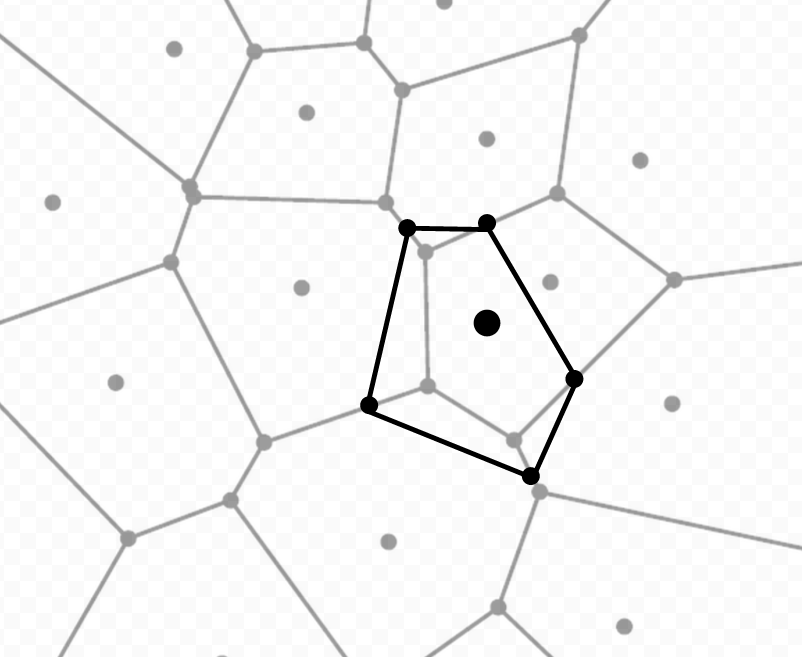
\includegraphics[width=7cm]{vd.png}
\end{center}
\caption{Eine neue Voronoi Region}
\end{figure}
\end{task}
\end{document}